\chapter{ObjetBDD - accéder aux bases de données}\label{objetbdd}

\section{Présentation}

ObjetBDD est une classe qui sert d'interface entre l'application et la base de données. Elle a été créée pour simplifier les requêtes, seules celles d'interrogation spécifiques devront être écrites.

Historiquement, ObjetBDD travaillait avec ADODB, une classe qui encapsulait la connexion à la base de données. Avec la sortie de PDO, la classe a été adaptée pour utiliser des connexions PDO.
Elle était également prévue pour fonctionner initialement avec Sybase ASE et MySQL. Les récentes évolutions ont porté sur le support des bases PostgreSQL : il n'est pas certain que toutes les fonctionnalités soient disponibles pour MySQL ou Sybase ASE.

Les fonctions initiales ont été modifiées ou complétées pour supporter maintenant les requêtes préparées.

\section{Fonctionnalités générales}
\subsection{Formatage des dates}
Les dates stockées dans les bases de données sont dans un format difficilement utilisable. La classe transforme automatiquement les dates dans le format français par défaut (mais d'autres formats possibles). 

Elle est également capable de transformer les dates reçues du navigateur au format de stockage. Le format de saisie est libre : la plupart des séparateurs sont supportés, l'année est rajoutée automatiquement, etc.

Le formatage des date inclut également les dates/heures.

\subsection{Opérations d'écriture en base de données}

La classe dispose de deux fonctions pour écrire les informations : ecrire() et supprimer(). La fonction ecrire() va décider s'il faut réaliser un insert ou un update, en fonction de la clé fournie. Par convention, si la clé vaut 0, un insert sera réalisé.

\subsection{Gestion des erreurs}

En cas d'échec d'exécution d'une requête SQL, la classe génère une exception.

\section{Variables générales utilisables}

Ces variables sont toutes publiques.
\begin{longtable}{|p{3cm}|c|p{8.5cm}|}
\hline
\textbf{Variable} & \textbf{Type} & \textbf{Signification} \\
\hline
\endhead
connection & PDO & instance PDO. Peut être utilisée pour instancier une nouvelle classe basée sur ObjetBDD à l'intérieur d'une fonction \\
\hline
id\_auto & entier & Si à 1, la classe gère la création automatique des identifiants. Si à 2, l'identifiant est généré manuellement, avec une requête de type \textit{max(id)} \\
\hline
formatDate & entier & 0 : amj, 1 : jma (défaut), 2 : mja \\
\hline
debug\_mode & entier & 0 : pas de mode de débogage, 1 : affichage des messages d'erreur, 2 : affichage de toutes les commandes SQL générées
\\
\hline
error\_data & tableau & liste de toutes les erreurs détectées lors de la vérification des données.  \\
 & & \$errorData[]["code"] : code d'erreur : \\
	& & 0 : non précisé \\
	& & 1 : champ non numérique \\
	& & 2 : champ texte trop grand \\
	& & 3 : masque (pattern) non conforme \\
	& & 4 : champ obligatoire vide \\
	& & \$errorData[]["colonne"] : champ concerne \\
	& & \$errorData[]["valeur"] : valeur initiale \\
\hline
srid & numérique & Valeur du srid pour les variables de type Postgis \\
\hline
quoteIdentifier & caractère & caractère utilisé pour encadrer les noms des colonnes dans les requêtes (pour les colonnes contenant une majuscule ou un accent) \\
\hline
transformComma & entier & Si à 1 (défaut), les virgules sont transformées en points pour les nombres décimaux \\
\hline

\caption{Liste des variables utilisables dans ObjetBDD}

\end{longtable}

En principe, les variables sont initialisées lors de l'instanciation de la classe, mais peuvent être modifiées à la volée, si nécessaire.

La classe est conçue pour fonctionner en UTF8.

\section{Héritage}

La classe ObjetBDD n'est pas instanciable, et doit donc être héritée. En particulier, le constructeur de la classe doit être surchargé pour rendre la classe opérante. 

\section{Fonctions principales}
\subsection{Constructeur de la classe}

\begin{lstlisting}
function __construct(PDO &$p_connection, array $param = array())
\end{lstlisting}
\subsubsection{Paramètres}
La fonction doit recevoir une instance PDO, correspondant à une connexion déjà réalisée à la base de données. Cette instance PDO est stockée ensuite dans la variable \textit{connection}, qui peut être réutilisée si d'autres classes héritées sont à instancier à l'intérieur du code.

Le tableau \textit{param} comprend, si nécessaire, l'ensemble des variables globales à mettre à jour.

\subsubsection{Surcharge}

Le constructeur doit être impérativement être surchargé, avec le code minimal suivant (exemple) : 

\begin{lstlisting}
function __construct($bdd, $param = array()) {
		$this->table = "acllogin";
		$this->colonnes = array (
				"acllogin_id" => array (
						"type" => 1,
						"key" => 1,
						"requis" => 1,
						"defaultValue" => 0 
				),
				"login" => array (
						"requis" => 1 
				),
				"logindetail" => array (
						"type" => 0,
						"requis" => 1 
				) 
		);
		parent::__construct ( $bdd, $param );
	}
\end{lstlisting}

\textit{table} doit correspondre au nom de la table (sans tenir compte du schéma, traité lors de la connexion à la base de données).

\textit{colonnes} contient la description des colonnes de la table. Chaque colonne doit être nommée, et contient un tableau, dont les  attributs possibles sont les suivants :

\begin{longtable}{|p{3cm}|p{10cm}|}
\hline
\textbf{Variable} & \textbf{Signification} \\
\hline
\endhead
type & 0 : varchar \\
& 1 : numérique (y compris décimaux) \\
& 2 : date \\
& 3 : datetime \\
& 4 : champ Postgis \\
\hline
requis & Si à 1, le contenu doit être fourni pour réaliser l'écriture \\
\hline
key & Si à 1, l'attribut est utilisé comme clé primaire (en principe, n'utiliser que des clés mono-attributs, même si la classe devrait être capable de gérer des clés multiples) \\
\hline
defaultValue & valeur par défaut. Il est possible d'indiquer le nom d'une fonction (entre guillemets). Parmi celles-ci, il est possible d'utiliser :\\
& getDateJour : retourne la date du jour \\
& getDateHeure : retourne la date et l'heure courante \\
& getLogin : retourne la valeur de la variable \$\_SESSION["login"]\\
\hline
parentAttrib & si vaut 1, la valeur est utilisée comme clé étrangère principale de l'enregistrement \\
\hline
longueur & pour les champs de type varchar, indique la longueur maximale autorisée (attention au codage UTF-8, les caractères accentués étant comptés pour 2) \\
\hline
pattern & pattern traité par expression régulière, pour tester la correspondance de l'information fournie au modèle décrit \\
\hline

\caption{Liste des attributs permettant de décrire les colonnes de la table\label{objetbdd-attr}}

\end{longtable}

Les deux derniers attributs sont toujours utilisables, mais en rarement employés.

\subsection{lire}
\begin{lstlisting}
lire($id, $getDefault = true, $parentValue = 0)
\end{lstlisting}

Fonction permettant de récupérer un enregistrement. Elle accepte les paramètres suivants :
\begin{longtable}{|p{3cm}|p{10cm}|}
\hline
\textbf{Variable} & \textbf{Signification} \\
\hline
\endhead
id & clé de l'enregistrement \\
\hline
getDefault & si à \textit{true}, récupère les valeurs par défaut si l'enregistrement n'existe pas dans la base (initialisation d'une saisie, par exemple)\\
\hline
parentValue & clé de l'enregistrement parent. Si \textit{getDefault} vaut \textit{true}, pré-remplit l'attribut qui contient la valeur \textit{parentAttrib} avec la clé fournie dans \textit{parentValue} \\
\hline

\caption{Liste des paramètres de la fonction lire}
\end{longtable}

La fonction retourne le tableau associatif correspondant.

\subsection{ecrire}
\begin{lstlisting}
ecrire($data)
\end{lstlisting}
Déclenche l'écriture des informations dans la base de données. \$data doit être un tableau qui comprend les attributs à écrire (au minimum, les attributs déclarés comme obligatoires).

Le nom des attributs fournis doit correspondre exactement au nom des colonnes.

En principe, ce tableau correspond à la variable \$\_REQUEST.

La fonction génère soit une commande insert, soit une commande update. En principe, la commande insert est générée si la clé fournie vaut 0.

Elle retourne la clé modifiée ou créée.

\subsection{supprimer}

\begin{lstlisting}
supprimer($id)
\end{lstlisting}

Permet de supprimer un enregistrement, à partir de sa clé. Attention : la fonction ne gère pas les suppressions en cascade, si ce n'est pas prévu directement dans la base de données.

\subsection{supprimerChamp}

\begin{lstlisting}
supprimerChamp($id, $champ)
\end{lstlisting}

Fonction très pratique pour supprimer tous les enregistrements fils. Elle génère une requête du type :
\begin{lstlisting}
delete from table where :champ = :id;
\end{lstlisting}


\subsection{getListe}

\begin{lstlisting}
getListe($order = "")
\end{lstlisting}

Fonction récupérant l'ensemble des enregistrements d'une table, triés ou non selon le contenu de la variable \$order.

\subsection{getListFromParent}

\begin{lstlisting}
function getListFromParent($parentId, $order = "")
\end{lstlisting}

Retourne la liste des enregistrements fils correspondant à la clé étrangère \$parentId. Le résultat peut ou non être trié selon les paramètres définis dans la seconde variable.

\subsection{getListParamAsPrepared}

\begin{lstlisting}
function getListeParamAsPrepared($sql, $data)
\end{lstlisting}

Permet de récupérer une liste d'enregistrements à partir de la requête SQL fournie et du tableau des données à insérer (requêtes préparées PDO), avec transformation des dates

\subsection{getListeParam}
\begin{lstlisting}
function getListeParam($sql)
\end{lstlisting}

Exécute la requête et retourne la liste des enregistrements correspondants, avec transformation des dates.

Attention : cette fonction ne gère pas la préparation des requêtes : il importe au codeur d'en tenir compte pour éviter les risques d'injection de code. Elle ne devrait être utilisée que dans les cas où une requête préparée ne peut être utilisée.

\subsection{ecrireTableNN}

\begin{lstlisting}
ecrireTableNN($nomTable, $nomCle1, $nomCle2, $id, $lignes)
\end{lstlisting}

Fonction permettant de mettre à jour les tables de relation NN, selon le schéma suivant :

\begin{figure}[H]
\centering
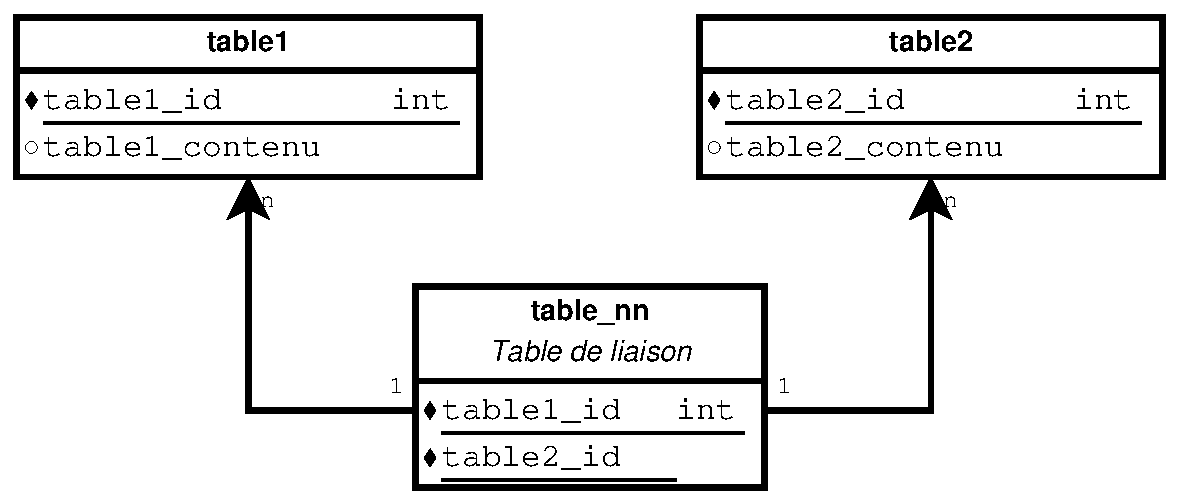
\includegraphics[width=0.8\linewidth]{dessin/schema-nn}
\caption{Structure d'une liaison N-N}
\end{figure}

En général, la saisie de ce type de liaisons est effectuée par des cases à cocher, ce qui permet de récupérer un tableau contenant la liste des clés de la table2 (champs html \textit{<input type checkbox name="attribut[]">}).

Les arguments à indiquer sont les suivants :
\begin{longtable}{|p{3cm}|p{10cm}|}
\hline
\textbf{Variable} & \textbf{Signification} \\
\hline
\endhead
nomTable & Nom de la table NN (table\_nn dans notre exemple) \\
\hline
nomCle1 & nom de l'attribut contenant la clé de la table principale \\
\hline
nomCle2 & nom de l'attribut contenant les clés de la table secondaire \\
\hline
id & valeur de la clé de la table principale \\
\hline
lignes & tableau contenant les valeurs de la table secondaire à conserver ou à rajouter \\
\hline

\caption{Liste des paramètres de la fonction ecrireTableNN}
\end{longtable}

La fonction ne génère que les requêtes de modification nécessaires (insertion ou suppression). Elle permet d'éviter de déclarer une instanciation d'ObjetBDD pour la table\_nn.

\subsection{getBlobReference}

\begin{lstlisting}
function getBlobReference($id, $fieldName)
\end{lstlisting}

Fonction permettant de récupérer un champ binaire stocké dans la base de données. PDO retourne l'identifiant interne PHP du fichier temporaire contenant l'information binaire lu.

Arguments :
\begin{longtable}{|p{3cm}|p{10cm}|}
\hline
\textbf{Variable} & \textbf{Signification} \\
\hline
\endhead
id & Clé de l'enregistrement \\
\hline
fieldName & nom de la colonne contenant l'information binaire \\
\hline
\caption{Liste des paramètres de la fonction getBlobReference}
\end{longtable}

\subsection{encodeData}

\begin{lstlisting}
encodeData($data)
\end{lstlisting}

Fonction encodant les quottes comprises dans les champs du tableau data, pour toutes les requêtes SQL directes (exécution ne passant pas par le mécanisme des requêtes préparées).

\subsection{executeAsPrepared}

\begin{lstlisting}
function executeAsPrepared($sql, $data, $onlyExecute = false) 
\end{lstlisting}

Fonction exécutant la requête fournie sous forme de requête préparée. Les variables à insérer sont décrites dans le tableau \textit{data}. Si l'attribut \$onlyExecute vaut true, la fonction ne retourne pas de résultat.

\subsection{executeSQL}

\begin{lstlisting}
function executeSQL($ls_sql) {
\end{lstlisting}

Exécute la commande SQL, sans précaution particulière (attention aux risques d'injection).

\subsection{formatDateDBversLocal}

\begin{lstlisting}
function formatDateDBversLocal($date, $type = 2)
\end{lstlisting}

Transforme la date, au format de la base de données, vers le format lisible pour l'utilisateur.

Si \$type vaut 3, la fonction retourne le champ au format date/heure.

\subsection{formatDateLocaleVersDB}
\begin{lstlisting}
function formatDateLocaleVersDB($date, $type = 2)
\end{lstlisting}

Transforme la date fournie en format géré par la base de données. Si le type vaut 3, un champ de type date/heure est attendu.

\subsection{utilDatesDBVersLocale}
\begin{lstlisting}
function utilDatesDBVersLocale($data)
\end{lstlisting}

Transforme les dates présentes dans le tableau joint à un format lisible par l'utilisateur.

\begin{lstlisting}
function utilDatesLocaleVersDB($data)
\end{lstlisting}

Transforme les dates présentes dans le tableau joint au format supporté par la base de données.

\section{Utilisation avancée}
\subsection{Requête multi-table contenant des champs date}
Un des cas fréquents posé par ObjetBDD est celui des requêtes manuelles qui retournent des dates. L'objectif est de les formater pour les mettre dans le même état que les dates décrites dans la table associée à la classe.

Le plus simple consiste à rajouter la colonne date complémentaire à la liste des variables juste avant d'exécuter la requête. Voici un exemple :
\begin{lstlisting}
$sql = "select t1.id, t1.date1, t2.id2, t2.date2
from table1 t1
join table2 t2 using (id)";
$this->colonnes["date2"]=array("type"=>2);
return $this->getListeParam($sql);
\end{lstlisting}

Une fois le contenu de la requête récupéré, la classe pourra alors appliquer la transformation de date sur la colonne issue de la  seconde table.

\section{Le tableau de paramètres ObjetBDDParam}\label{objetbddparam}

ObjetBDDParam est une variable contenant les paramètres par défaut utilisés pour initialiser les instances issues d'ObjetBDD. C'est en particulier assez pratique pour gérer le choix de la langue d'affichage pour les dates. Il est également possible de modifier, de manière globale dans le logiciel, le fonctionnement d'ObjetBDD.

Ce tableau devrait être passé systématiquement en paramètre de toute instanciation d'objet basé sur ObjetBDD.

\chapter{Exécuter les actions}
Le framework est conçu pour n'exécuter que les actions décrites dans un fichier XML (\textit{cf.} \ref{labelxml} \textit{\nameref{labelxml}}, page \pageref{labelxml}).

Les actions sont identifiées par deux informations : d'une part, le nom du fichier PHP à exécuter, et d'autre part un paramètre permettant de décrire ce qu'il faut réaliser précisément. Ce second paramètre pourrait ne pas être utilisé, mais cela impliquerait un fichier par action. 
Le framework a été conçu pour obtenir un bon équilibre entre le nombre de fichiers et la navigation dans le code.

\section{Les actions standard}

En général, on identifie facilement les actions suivants sur un type d'objet :
\begin{itemize}
\item l'affichage d'une boite de recherche et de la liste des dossiers correspondants ;
\item l'affichage du détail d'un enregistrement ;
\item l'affichage de la page permettant de créer ou de modifier un enregistrement ;
\item l'écriture des informations en base de données ;
\item la suppression d'une fiche.
\end{itemize}

Par convention, ces actions sont nommées \textbf{list}, \textbf{display}, \textbf{change}, \textbf{write} et \textbf{delete}. 

Voici un exemple de code standard utilisé pour traiter tous les modules (fichier modules/example/example.php, à recopier et à adapter...) :

\begin{lstlisting}
include_once 'modules/example/example.class.php';
$dataClass = new Example($bdd,$ObjetBDDParam);
$keyName = "example_id";
$id = $_REQUEST[$keyName];

switch ($t_module["param"]) {
	case "list":
		/*
		 * Display the list of all records of the table
		 */
		 /*
		 * $searchExample must be defined into modules/beforesession.inc.php :
		 * include_once 'modules/classes/searchParam.class.php';
		 * and into modules/common.inc.php :
		 * if (!isset($_SESSION["searchExample"])) {
    	 * $searchExample = new SearchExample();
		 *	$_SESSION["searchExample"] = $searchExample; 
		 *	} else {
		 *	$searchExample = $_SESSION["searchExample"];
		 *	}
		 * and, also, into modules/classes/searchParam.class.php...
		 */
		 $searchExample->setParam ( $_REQUEST );
		 $dataSearch = $searchExample->getParam ();
		if ($searchExample->isSearch () == 1) {
			$data = $dataClass->getListeSearch ( $dataExample );		
		$vue->set($data , "data");
		$vue->set(1, "isSearch");
		}
		$vue->set($dataSearch, "exampleSearch");
		$vue->set("example/exampleList.tpl","corps" );
		break;
	case "display":
		/*
		 * Display the detail of the record
		 */
		$data = $dataClass->lire($id);
		$vue->set($data,"data");
		/*
		 * Assignation du modele d'affichage
		 */
		$vue->set(  "example/exampleDisplay.tpl", "corps");

		break;
	case "change":
		/*
		 * open the form to modify the record
		 * If is a new record, generate a new record with default value :
		 * $_REQUEST["idParent"] contains the identifiant of the parent record 
		 */
		dataRead($dataClass, $id, "example/exampleChange.tpl", $_REQUEST["idParent"]);
		break;
	case "write":
		/*
		 * write record in database
		 */
		$id = dataWrite($dataClass, $_REQUEST);
		if ($id > 0) {
			$_REQUEST[$keyName] = $id;
		}
		break;
	case "delete":
		/*
		 * delete record
		 */
		dataDelete($dataClass, $id);
		break;
}
\end{lstlisting}

Quelques explications...

Le code commence par charger la classe héritée d'ObjetBDD, puis celle-ci est instanciée avec, en paramètres, la connexion PDO à utiliser et le tableau \textit{ObjetBDDParam}, qui contient la configuration par défaut d'ObjetBDD (\textit{cf.} \ref{objetbddparam} \textit{\nameref{objetbddparam}}, page \pageref{objetbddparam}).

Le nom de la clé associée est indiqué, ce qui permet d'obtenir une code plus générique.

Ensuite, le tableau contenant la description de l'action (t\_param) est analysé, et plus particulièrement sa valeur \textit{param}, qui correspond à ce qu'on attend du module, avec une instruction \textit{switch}.

Quelques précisions sur ce qui est implémenté par défaut.

\subsection{list}

Permet d'afficher une boite de recherche et la liste des dossiers associés. 

\subsubsection{La classe de gestion des critères de recherche}

Les paramètres de recherche peuvent être stockés en variable de session, pour que l'utilisateur récupère la liste des dossiers affichés précédemment quand il revient sur cet écran. 

Chaque jeu de paramètres est déclaré dans une instance héritée de la classe \textit{SearchParam}, dans le fichier \textit{modules/classes/search.class.php}.

Voici un exemple d'instanciation de cette classe de recherche :
\begin{lstlisting}
class SearchExample extends SearchParam {
	function __construct() {
		$this->param = array (
				"comment" => "",
				"numero" => 0,
				"numero1" => "",
				"dateExample" => date ( 'd/m/Y' ) 
		);
		$this->paramNum = array (
				"numero",
				"numero1" 
		);
		parent::__construct ();
	}
}
\end{lstlisting}

Deux tableaux doivent être déclarés. Le premier correspond aux attributs utilisables dans la recherche, et leur valeur par défaut doit être indiquée. Le second indique quels sont les champs qui sont numériques.

Deux fonctions sont utilisés couramment : 
\begin{itemize}
\item setParam(\$\_REQUEST) : met à jour les paramètres de recherche ;
\item getParam() : retourne le tableau avec les paramètres de recherche.
\end{itemize}

De plus, une fonction utilitaire permet de savoir s'il s'agit de la première fois que la recherche est utilisée. Si le formulaire contient un champ configuré ainsi :
\begin{lstlisting}
<input type="hidden" name="isSearch" value="1">
\end{lstlisting}
Il est alors facile de savoir si le formulaire de recherche a déjà ou non été appelé (la variable \textit{isSearch} est initialisée à 0).

\subsubsection{Affichage de la liste}
L'affichage de la liste va être traité par la vue Smarty. Le contenu va être transmis (par convention, dans une variable nommée \textit{data}, mais dans certains cas, il vaut mieux utiliser d'autres libellés, surtout si plusieurs informations doivent être affichées en parallèle).

Il est important également de transmettre le nom du \textit{template} qui devra être utilisé, en assignant la valeur à la variable normalisée \textit{corps}.

\subsection{display}

L'entrée \textit{display} permet d'afficher le détail des informations relatives à un enregistrement. Le fonctionnement est beaucoup plus simple que pour l'affichage de la liste : il suffit de transmettre à la vue le contenu de l'enregistrement lu à partir d'ObjetBDD.

Toutefois, si la table contient de nombreuses tables filles, il faudra adapter le code pour transmettre également à la vue l'ensemble des listes d'informations associées.

\subsection{change}

Cette entrée va déclencher l'affichage du formulaire de modification. Par défaut, si la clé vaut 0, on considère qu'il s'agit d'une création.

Pour simplifier l'écriture, une fonction générique est utilisée : 

\begin{lstlisting}
dataRead($dataClass, $id, "example/exampleChange.tpl", $_REQUEST["idParent"]);
\end{lstlisting}

Cette fonction va réaliser automatiquement la lecture de l'information dans la classe ObjetBDD. Si la clé vaut 0, les valeurs par défaut seront récupérées. S'il s'agit d'une table fille, la valeur de la clé parente sera également ajoutée, si la classe a été décrite en ce sens (\textit{cf.} \ref{objetbdd-attr} \textit{\nameref{objetbdd-attr}}, page \pageref{objetbdd-attr}).

Le troisième paramètre correspond au nom du \textit{template} Smarty à utiliser, qui sera assigné automatiquement.

\subsection{write}
Cette entrée est celle qui est utilisée pour traiter les écritures en base de données. Elle utilise également une fonction générique : 
\begin{lstlisting}
$id = dataWrite($dataClass, $_REQUEST);
\end{lstlisting}

Cette fonction gère l'écriture dans la base de données, traite les erreurs, et retourne l'identifiant, qui doit être supérieur à 0 si l'opération a aboutit.

Une fois l'écriture réalisée, la valeur de l'identifiant est mise à jour, pour que le module appelé après dispose de la bonne valeur (affichage du détail après une création, par exemple).

\subsection{delete}
Cette dernière opération, qui traite la suppression d'un enregistrement, utilise également une fonction générique :

\begin{lstlisting}
dataDelete($dataClass, $id);
\end{lstlisting}

Cette fonction gère également les erreurs et les enchaînements en fonction du résultat de l'opération.

Attention : le framework n'a pas été conçu pour gérer les suppressions en cascade. Il faut donc soit coder les effacements dans les tables filles à partir d'une surcharge de la fonction \textit{supprimer()} d'ObjetBDD, soit configurer la base de données pour qu'elle réalise l'opération elle-même.